% Options for packages loaded elsewhere
\PassOptionsToPackage{unicode}{hyperref}
\PassOptionsToPackage{hyphens}{url}
%
\documentclass[
]{article}
\usepackage{amsmath,amssymb}
\usepackage{lmodern}
\usepackage{ifxetex,ifluatex}
\ifnum 0\ifxetex 1\fi\ifluatex 1\fi=0 % if pdftex
  \usepackage[T1]{fontenc}
  \usepackage[utf8]{inputenc}
  \usepackage{textcomp} % provide euro and other symbols
\else % if luatex or xetex
  \usepackage{unicode-math}
  \defaultfontfeatures{Scale=MatchLowercase}
  \defaultfontfeatures[\rmfamily]{Ligatures=TeX,Scale=1}
\fi
% Use upquote if available, for straight quotes in verbatim environments
\IfFileExists{upquote.sty}{\usepackage{upquote}}{}
\IfFileExists{microtype.sty}{% use microtype if available
  \usepackage[]{microtype}
  \UseMicrotypeSet[protrusion]{basicmath} % disable protrusion for tt fonts
}{}
\makeatletter
\@ifundefined{KOMAClassName}{% if non-KOMA class
  \IfFileExists{parskip.sty}{%
    \usepackage{parskip}
  }{% else
    \setlength{\parindent}{0pt}
    \setlength{\parskip}{6pt plus 2pt minus 1pt}}
}{% if KOMA class
  \KOMAoptions{parskip=half}}
\makeatother
\usepackage{xcolor}
\IfFileExists{xurl.sty}{\usepackage{xurl}}{} % add URL line breaks if available
\IfFileExists{bookmark.sty}{\usepackage{bookmark}}{\usepackage{hyperref}}
\hypersetup{
  pdftitle={SEIRD contact matrix},
  hidelinks,
  pdfcreator={LaTeX via pandoc}}
\urlstyle{same} % disable monospaced font for URLs
\usepackage[margin=1in]{geometry}
\usepackage{color}
\usepackage{fancyvrb}
\newcommand{\VerbBar}{|}
\newcommand{\VERB}{\Verb[commandchars=\\\{\}]}
\DefineVerbatimEnvironment{Highlighting}{Verbatim}{commandchars=\\\{\}}
% Add ',fontsize=\small' for more characters per line
\usepackage{framed}
\definecolor{shadecolor}{RGB}{248,248,248}
\newenvironment{Shaded}{\begin{snugshade}}{\end{snugshade}}
\newcommand{\AlertTok}[1]{\textcolor[rgb]{0.94,0.16,0.16}{#1}}
\newcommand{\AnnotationTok}[1]{\textcolor[rgb]{0.56,0.35,0.01}{\textbf{\textit{#1}}}}
\newcommand{\AttributeTok}[1]{\textcolor[rgb]{0.77,0.63,0.00}{#1}}
\newcommand{\BaseNTok}[1]{\textcolor[rgb]{0.00,0.00,0.81}{#1}}
\newcommand{\BuiltInTok}[1]{#1}
\newcommand{\CharTok}[1]{\textcolor[rgb]{0.31,0.60,0.02}{#1}}
\newcommand{\CommentTok}[1]{\textcolor[rgb]{0.56,0.35,0.01}{\textit{#1}}}
\newcommand{\CommentVarTok}[1]{\textcolor[rgb]{0.56,0.35,0.01}{\textbf{\textit{#1}}}}
\newcommand{\ConstantTok}[1]{\textcolor[rgb]{0.00,0.00,0.00}{#1}}
\newcommand{\ControlFlowTok}[1]{\textcolor[rgb]{0.13,0.29,0.53}{\textbf{#1}}}
\newcommand{\DataTypeTok}[1]{\textcolor[rgb]{0.13,0.29,0.53}{#1}}
\newcommand{\DecValTok}[1]{\textcolor[rgb]{0.00,0.00,0.81}{#1}}
\newcommand{\DocumentationTok}[1]{\textcolor[rgb]{0.56,0.35,0.01}{\textbf{\textit{#1}}}}
\newcommand{\ErrorTok}[1]{\textcolor[rgb]{0.64,0.00,0.00}{\textbf{#1}}}
\newcommand{\ExtensionTok}[1]{#1}
\newcommand{\FloatTok}[1]{\textcolor[rgb]{0.00,0.00,0.81}{#1}}
\newcommand{\FunctionTok}[1]{\textcolor[rgb]{0.00,0.00,0.00}{#1}}
\newcommand{\ImportTok}[1]{#1}
\newcommand{\InformationTok}[1]{\textcolor[rgb]{0.56,0.35,0.01}{\textbf{\textit{#1}}}}
\newcommand{\KeywordTok}[1]{\textcolor[rgb]{0.13,0.29,0.53}{\textbf{#1}}}
\newcommand{\NormalTok}[1]{#1}
\newcommand{\OperatorTok}[1]{\textcolor[rgb]{0.81,0.36,0.00}{\textbf{#1}}}
\newcommand{\OtherTok}[1]{\textcolor[rgb]{0.56,0.35,0.01}{#1}}
\newcommand{\PreprocessorTok}[1]{\textcolor[rgb]{0.56,0.35,0.01}{\textit{#1}}}
\newcommand{\RegionMarkerTok}[1]{#1}
\newcommand{\SpecialCharTok}[1]{\textcolor[rgb]{0.00,0.00,0.00}{#1}}
\newcommand{\SpecialStringTok}[1]{\textcolor[rgb]{0.31,0.60,0.02}{#1}}
\newcommand{\StringTok}[1]{\textcolor[rgb]{0.31,0.60,0.02}{#1}}
\newcommand{\VariableTok}[1]{\textcolor[rgb]{0.00,0.00,0.00}{#1}}
\newcommand{\VerbatimStringTok}[1]{\textcolor[rgb]{0.31,0.60,0.02}{#1}}
\newcommand{\WarningTok}[1]{\textcolor[rgb]{0.56,0.35,0.01}{\textbf{\textit{#1}}}}
\usepackage{graphicx}
\makeatletter
\def\maxwidth{\ifdim\Gin@nat@width>\linewidth\linewidth\else\Gin@nat@width\fi}
\def\maxheight{\ifdim\Gin@nat@height>\textheight\textheight\else\Gin@nat@height\fi}
\makeatother
% Scale images if necessary, so that they will not overflow the page
% margins by default, and it is still possible to overwrite the defaults
% using explicit options in \includegraphics[width, height, ...]{}
\setkeys{Gin}{width=\maxwidth,height=\maxheight,keepaspectratio}
% Set default figure placement to htbp
\makeatletter
\def\fps@figure{htbp}
\makeatother
\setlength{\emergencystretch}{3em} % prevent overfull lines
\providecommand{\tightlist}{%
  \setlength{\itemsep}{0pt}\setlength{\parskip}{0pt}}
\setcounter{secnumdepth}{-\maxdimen} % remove section numbering
\ifluatex
  \usepackage{selnolig}  % disable illegal ligatures
\fi
\newlength{\cslhangindent}
\setlength{\cslhangindent}{1.5em}
\newlength{\csllabelwidth}
\setlength{\csllabelwidth}{3em}
\newenvironment{CSLReferences}[2] % #1 hanging-ident, #2 entry spacing
 {% don't indent paragraphs
  \setlength{\parindent}{0pt}
  % turn on hanging indent if param 1 is 1
  \ifodd #1 \everypar{\setlength{\hangindent}{\cslhangindent}}\ignorespaces\fi
  % set entry spacing
  \ifnum #2 > 0
  \setlength{\parskip}{#2\baselineskip}
  \fi
 }%
 {}
\usepackage{calc}
\newcommand{\CSLBlock}[1]{#1\hfill\break}
\newcommand{\CSLLeftMargin}[1]{\parbox[t]{\csllabelwidth}{#1}}
\newcommand{\CSLRightInline}[1]{\parbox[t]{\linewidth - \csllabelwidth}{#1}\break}
\newcommand{\CSLIndent}[1]{\hspace{\cslhangindent}#1}

\title{SEIRD contact matrix}
\author{}
\date{\vspace{-2.5em}}

\begin{document}
\maketitle

\hypertarget{introduction}{%
\subsection{Introduction}\label{introduction}}

Age-structured compartmental models such as the SEIRD implemented in
comomodels use contact matrices to specify the spread of a disease
within and between age groups. Given a contact matrix \(C\), each
element \(C_{i,j}\) indicates the expected number of contacts someone
from age group \(i\) has per day with people from age group \(j\).

Comomodels includes estimates of the contact matrix for each country
((Prem et al. 2021); with full details available in the data
documentation). Separate matrices are available for contacts at home,
work, school, and other. Below, we generate a plot of the contact
matrices.

\begin{Shaded}
\begin{Highlighting}[]
\FunctionTok{library}\NormalTok{(comomodels)}
\FunctionTok{library}\NormalTok{(tidyverse)}
\FunctionTok{library}\NormalTok{(ggplot2)}
\FunctionTok{library}\NormalTok{(socialmixr)}
\end{Highlighting}
\end{Shaded}

\begin{Shaded}
\begin{Highlighting}[]
\NormalTok{contact\_home }\OtherTok{\textless{}{-}}\NormalTok{ comomodels}\SpecialCharTok{::}\NormalTok{contact\_home}
\NormalTok{contact\_work }\OtherTok{\textless{}{-}}\NormalTok{ comomodels}\SpecialCharTok{::}\NormalTok{contact\_work}
\NormalTok{contact\_school }\OtherTok{\textless{}{-}}\NormalTok{ comomodels}\SpecialCharTok{::}\NormalTok{contact\_school}
\NormalTok{contact\_other }\OtherTok{\textless{}{-}}\NormalTok{ comomodels}\SpecialCharTok{::}\NormalTok{contact\_other}
\NormalTok{population }\OtherTok{\textless{}{-}}\NormalTok{ comomodels}\SpecialCharTok{::}\NormalTok{population}
\end{Highlighting}
\end{Shaded}

\begin{Shaded}
\begin{Highlighting}[]
\CommentTok{\# reformat matrices for plotting}
\NormalTok{ages }\OtherTok{\textless{}{-}} \FunctionTok{seq}\NormalTok{(}\DecValTok{0}\NormalTok{, }\DecValTok{80}\NormalTok{, }\DecValTok{5}\NormalTok{)}
\NormalTok{age\_names }\OtherTok{\textless{}{-}} \FunctionTok{vector}\NormalTok{(}\AttributeTok{length =} \DecValTok{16}\NormalTok{)}
\ControlFlowTok{for}\NormalTok{(i }\ControlFlowTok{in} \FunctionTok{seq\_along}\NormalTok{(age\_names)) \{}
\NormalTok{  age\_names[i] }\OtherTok{\textless{}{-}} \FunctionTok{paste0}\NormalTok{(ages[i], }\StringTok{"{-}"}\NormalTok{, ages[i }\SpecialCharTok{+} \DecValTok{1}\NormalTok{])}
\NormalTok{\}}

\NormalTok{format\_matrix }\OtherTok{\textless{}{-}} \ControlFlowTok{function}\NormalTok{(contact\_matrix, age\_names) \{}
  \FunctionTok{colnames}\NormalTok{(contact\_matrix) }\OtherTok{\textless{}{-}}\NormalTok{ age\_names}
\NormalTok{  contact\_matrix}\SpecialCharTok{$}\NormalTok{age\_infectee }\OtherTok{\textless{}{-}}\NormalTok{ age\_names}
\NormalTok{  contact\_matrix }\SpecialCharTok{\%\textgreater{}\%}
    \FunctionTok{pivot\_longer}\NormalTok{(}\FunctionTok{all\_of}\NormalTok{(age\_names)) }\SpecialCharTok{\%\textgreater{}\%} 
    \FunctionTok{rename}\NormalTok{(}\AttributeTok{age\_infector=}\NormalTok{name) }\SpecialCharTok{\%\textgreater{}\%} 
    \FunctionTok{mutate}\NormalTok{(}\AttributeTok{age\_infector=}\FunctionTok{fct\_relevel}\NormalTok{(age\_infector, age\_names)) }\SpecialCharTok{\%\textgreater{}\%} 
    \FunctionTok{mutate}\NormalTok{(}\AttributeTok{age\_infectee=}\FunctionTok{fct\_relevel}\NormalTok{(age\_infectee, age\_names))}
\NormalTok{\}}

\NormalTok{c\_home }\OtherTok{\textless{}{-}} \FunctionTok{format\_matrix}\NormalTok{(contact\_home}\SpecialCharTok{$}\StringTok{"United Kingdom"}\NormalTok{, age\_names) }\SpecialCharTok{\%\textgreater{}\%} \FunctionTok{mutate}\NormalTok{(}\AttributeTok{type=}\StringTok{"home"}\NormalTok{)}
\NormalTok{c\_work }\OtherTok{\textless{}{-}} \FunctionTok{format\_matrix}\NormalTok{(contact\_work}\SpecialCharTok{$}\StringTok{"United Kingdom"}\NormalTok{, age\_names) }\SpecialCharTok{\%\textgreater{}\%} \FunctionTok{mutate}\NormalTok{(}\AttributeTok{type=}\StringTok{"work"}\NormalTok{)}
\NormalTok{c\_school }\OtherTok{\textless{}{-}} \FunctionTok{format\_matrix}\NormalTok{(contact\_school}\SpecialCharTok{$}\StringTok{"United Kingdom"}\NormalTok{, age\_names) }\SpecialCharTok{\%\textgreater{}\%} \FunctionTok{mutate}\NormalTok{(}\AttributeTok{type=}\StringTok{"school"}\NormalTok{)}
\NormalTok{c\_other }\OtherTok{\textless{}{-}} \FunctionTok{format\_matrix}\NormalTok{(contact\_other}\SpecialCharTok{$}\StringTok{"United Kingdom"}\NormalTok{, age\_names) }\SpecialCharTok{\%\textgreater{}\%} \FunctionTok{mutate}\NormalTok{(}\AttributeTok{type=}\StringTok{"other"}\NormalTok{)}

\NormalTok{c\_all }\OtherTok{\textless{}{-}}\NormalTok{ c\_home }\SpecialCharTok{\%\textgreater{}\%}
  \FunctionTok{bind\_rows}\NormalTok{(c\_work) }\SpecialCharTok{\%\textgreater{}\%} 
  \FunctionTok{bind\_rows}\NormalTok{(c\_school) }\SpecialCharTok{\%\textgreater{}\%} 
  \FunctionTok{bind\_rows}\NormalTok{(c\_other)}

\CommentTok{\# plot all}
\NormalTok{c\_all }\SpecialCharTok{\%\textgreater{}\%}
  \FunctionTok{ggplot}\NormalTok{(}\FunctionTok{aes}\NormalTok{(}\AttributeTok{x=}\NormalTok{age\_infector, }\AttributeTok{y=}\NormalTok{age\_infectee, }\AttributeTok{fill=}\NormalTok{value)) }\SpecialCharTok{+}
  \FunctionTok{geom\_tile}\NormalTok{() }\SpecialCharTok{+}
  \FunctionTok{scale\_fill\_viridis\_c}\NormalTok{() }\SpecialCharTok{+}
  \FunctionTok{facet\_wrap}\NormalTok{(}\SpecialCharTok{\textasciitilde{}}\NormalTok{type) }\SpecialCharTok{+}
  \FunctionTok{theme}\NormalTok{(}\AttributeTok{axis.text.x =} \FunctionTok{element\_text}\NormalTok{(}\AttributeTok{angle=}\DecValTok{90}\NormalTok{, }\AttributeTok{vjust=}\FloatTok{0.5}\NormalTok{, }\AttributeTok{hjust=}\DecValTok{1}\NormalTok{))}
\end{Highlighting}
\end{Shaded}

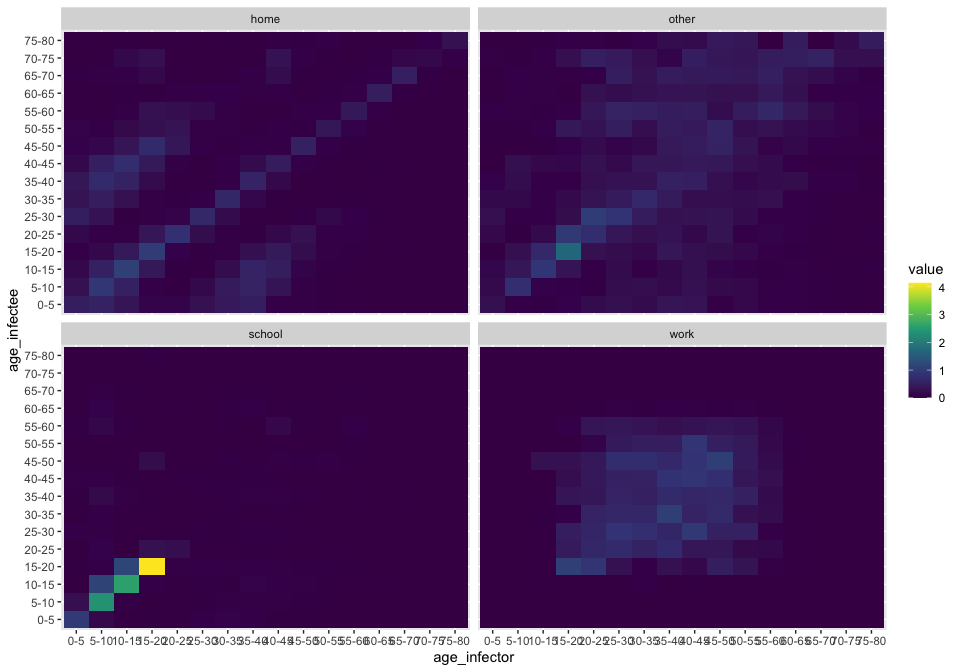
\includegraphics{SEIRD_contact_matrix_files/figure-latex/unnamed-chunk-3-1.pdf}

While it is possible to construct location-based transmission models, in
this study we consider only age structure. Thus, we obtain the total
contact matrix for the age-structured SEIRD model by summing the four
location specific contact matrices. Further details, including an
explanation of the model equations, can be found in the
SEIRD\_age\_structured vignette in the comomodels package:
\url{https://github.com/Como-DTC-Collaboration/como-models/blob/main/vignettes/SEIRD_age_structured.Rmd}

\hypertarget{uncertainty-in-the-contact-matrix}{%
\subsection{Uncertainty in the contact
matrix}\label{uncertainty-in-the-contact-matrix}}

Typically, when performing simulations of the age-structured SEIR model,
or inference for the parameters of the model, the contact matrix is
provided as a fixed input. However, using fixed values for the contact
matrix neglects the uncertainty which may be present in the contact
data.

The purpose of the remainder of this notebook is to investigate the
sensitivity of the outputs of the age-structured SEIRD model to the
values of the contact matrix. Using bootstrap samples which represent
the uncertainty in the contact matrix, we show significant uncertainty
in the numbers of infected individuals. The bootstrap algorithm works by
repeatedly selecting random samples (with replacement) of the survey
respondents, and using the sample to calculate a particular contact
matrix. Each sample yields a potentially different contact matrix, and
this set of contact matrices reveals something of the uncertainty in its
values.

\hypertarget{accuracy-of-uncertainty-estimates-produced-by-the-bootstrapping-methods}{%
\subsection{Accuracy of uncertainty estimates produced by the
bootstrapping
methods}\label{accuracy-of-uncertainty-estimates-produced-by-the-bootstrapping-methods}}

The bootstrap algorithm is an easy way to obtain some idea of the
uncertainty in the contact matrix. However, due to the simplicity of the
procedure, its results should be treated as mere approximations of the
true uncertainty that may exist in the contact matrix. In particular,
the bootstrap algorithm does not account for the possibility that the
contact data in the original survey is unrepresentative of the actual
population. For example, if contact data is collected primarily from an
urban area in a country whose population is mostly rural, the resulting
contact matrices may be inaccurate for the country, and the bootstrap
cannot account for the lack of information in the original data.

\hypertarget{bootstrap-samples-of-contact-matrices}{%
\subsection{Bootstrap samples of contact
matrices}\label{bootstrap-samples-of-contact-matrices}}

We obtain samples of the contact matrix using the socialmixr library
which accesses the POLYMOD data. This library allows us to generate
bootstrap samples of the contact matrix for countries covered by the
study. The first step is to generate 200 of these samples for the
contact matrix in the United Kingdom.

\begin{Shaded}
\begin{Highlighting}[]

\CommentTok{\# Define age groups and names}
\NormalTok{ages }\OtherTok{\textless{}{-}} \FunctionTok{seq}\NormalTok{(}\DecValTok{0}\NormalTok{, }\DecValTok{80}\NormalTok{, }\DecValTok{5}\NormalTok{)}
\NormalTok{age\_names }\OtherTok{\textless{}{-}} \FunctionTok{vector}\NormalTok{(}\AttributeTok{length =} \DecValTok{16}\NormalTok{)}
\ControlFlowTok{for}\NormalTok{(i }\ControlFlowTok{in} \FunctionTok{seq\_along}\NormalTok{(age\_names)) \{}
\NormalTok{  age\_names[i] }\OtherTok{\textless{}{-}} \FunctionTok{paste0}\NormalTok{(ages[i], }\StringTok{"{-}"}\NormalTok{, ages[i }\SpecialCharTok{+} \DecValTok{1}\NormalTok{])}
\NormalTok{\}}

\CommentTok{\# Get population data}
\NormalTok{pops }\OtherTok{\textless{}{-}}\NormalTok{ population[population}\SpecialCharTok{$}\NormalTok{country }\SpecialCharTok{==} \StringTok{"United Kingdom"}\NormalTok{, ]}\SpecialCharTok{$}\NormalTok{pop}
\NormalTok{pop\_fraction }\OtherTok{\textless{}{-}}\NormalTok{ pops}\SpecialCharTok{/}\FunctionTok{sum}\NormalTok{(pops)}
\NormalTok{pop\_fraction[}\DecValTok{16}\NormalTok{] }\OtherTok{\textless{}{-}} \FunctionTok{sum}\NormalTok{(pop\_fraction[}\DecValTok{16}\SpecialCharTok{:}\DecValTok{21}\NormalTok{])}
\NormalTok{pop\_fraction }\OtherTok{\textless{}{-}}\NormalTok{ pop\_fraction[}\DecValTok{1}\SpecialCharTok{:}\DecValTok{16}\NormalTok{]}
\NormalTok{n\_ages }\OtherTok{\textless{}{-}} \DecValTok{16}

\CommentTok{\# Load the contact matrix data from POLYMOD and get bootstrap samples}
\NormalTok{n\_bootstrap }\OtherTok{\textless{}{-}} \DecValTok{200}
\FunctionTok{data}\NormalTok{(polymod)}
\NormalTok{polymod\_data }\OtherTok{\textless{}{-}} \FunctionTok{contact\_matrix}\NormalTok{(polymod,}
                               \AttributeTok{n=}\NormalTok{n\_bootstrap,}
                               \AttributeTok{countries=}\StringTok{"United Kingdom"}\NormalTok{,}
                               \AttributeTok{age.limits=}\NormalTok{ages)}

\CommentTok{\# Get the first element of the list, which contains the matrices}
\NormalTok{matrices }\OtherTok{\textless{}{-}}\NormalTok{ polymod\_data[}\StringTok{"matrices"}\NormalTok{][[}\DecValTok{1}\NormalTok{]]}
\end{Highlighting}
\end{Shaded}

First, we inspect the range of values in the sampled contact matrices.
In the plot below, we look at the distribution of the diagonal elements
of the matrix for each age group.

\begin{Shaded}
\begin{Highlighting}[]

\NormalTok{contacts\_same\_age }\OtherTok{\textless{}{-}} \FunctionTok{c}\NormalTok{()}
\NormalTok{ages\_list }\OtherTok{\textless{}{-}} \FunctionTok{c}\NormalTok{()}
\ControlFlowTok{for}\NormalTok{ (i }\ControlFlowTok{in} \DecValTok{1}\SpecialCharTok{:}\NormalTok{n\_bootstrap)\{}
\NormalTok{  contacts\_same\_age }\OtherTok{\textless{}{-}} \FunctionTok{append}\NormalTok{(contacts\_same\_age, }\FunctionTok{diag}\NormalTok{(matrices[[i]][[}\DecValTok{1}\NormalTok{]])[}\DecValTok{1}\SpecialCharTok{:}\DecValTok{16}\NormalTok{])}
\NormalTok{  ages\_list }\OtherTok{\textless{}{-}} \FunctionTok{append}\NormalTok{(ages\_list, age\_names)}
\NormalTok{\}}

\NormalTok{data }\OtherTok{\textless{}{-}} \FunctionTok{data.frame}\NormalTok{(ages\_list, contacts\_same\_age)}
\NormalTok{data}\SpecialCharTok{$}\NormalTok{ages\_list }\OtherTok{\textless{}{-}} \FunctionTok{factor}\NormalTok{(data}\SpecialCharTok{$}\NormalTok{ages\_list, }\AttributeTok{levels=}\NormalTok{age\_names[}\DecValTok{1}\SpecialCharTok{:}\DecValTok{16}\NormalTok{], }\AttributeTok{ordered=}\ConstantTok{TRUE}\NormalTok{)}

\FunctionTok{ggplot}\NormalTok{(data, }\FunctionTok{aes}\NormalTok{(}\AttributeTok{x=}\NormalTok{ages\_list, }\AttributeTok{y=}\NormalTok{contacts\_same\_age), l) }\SpecialCharTok{+} \FunctionTok{geom\_boxplot}\NormalTok{() }\SpecialCharTok{+}
  \FunctionTok{xlab}\NormalTok{(}\StringTok{"Age group"}\NormalTok{) }\SpecialCharTok{+} \FunctionTok{ylab}\NormalTok{(}\StringTok{"Number of contacts with same age group"}\NormalTok{)}
\end{Highlighting}
\end{Shaded}

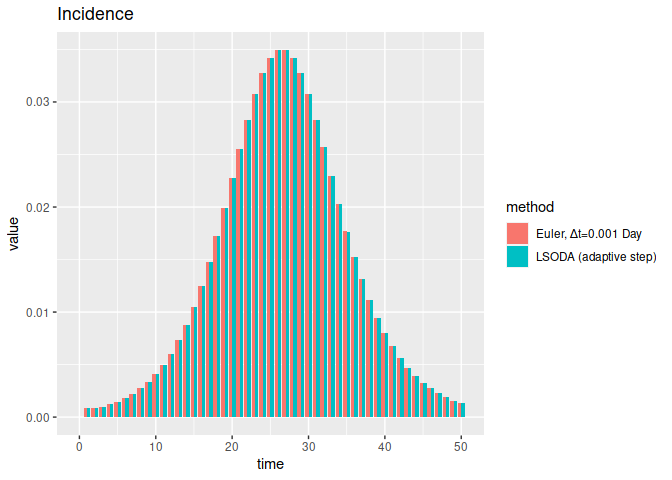
\includegraphics{SEIRD_contact_matrix_files/figure-latex/unnamed-chunk-5-1.pdf}

The plot shows the most uncertainty for ages 5--20 (schoolchildren). In
most of the other age groups, the uncertainty is small but nowhere does
it appear negligible. In the next section, the effect of these
uncertainties on the SEIR outputs will be studied.

\hypertarget{seird-simulations}{%
\subsection{SEIRD simulations}\label{seird-simulations}}

In this step, we run the age-structured SEIRD model once for each
bootstrap sample of the contact matrix. We use fixed values for the
other parameters of the model. We set an initial exposed group
compartment equal to 0.1\% of the population size, and all other
individuals in the susceptible group.

The transmission parameters are set to resemble those of the COVID-19
outbreak. For the latency period, we assume 5.5 days (Xin et al. 2021),
and for the duration of infectiousness, 2 days (thus, fewer than 1\% of
individuals are infectious after 10 days, in line with government
guidelines (UK government 2021)). To set the transmission rate
\(\beta\), we choose the value such that the basic reproduction number,
\(R_0\), is equal to 2.4 (Ferguson et al. 2020). The age-structured
model also takes the parameter \(\mu\) which specifies the rate at which
infected people enter the deceased compartment. For this parameter, we
provide a vector giving a separate value for each age group. The values
are selected to resemble the death rates of the COVID-19 outbreak in
mainland China during January and February 2020 (Verity et al. 2020). To
obtain estimates of \(\mu\) for each age group, we use data for the case
fatality ratio (IFR).

To calculate the recovery rate (\(\gamma\)) and the death rate (\(\mu\))
from the above quantities, we introduce \(\eta\) giving the inverse of
the average duration of infectiousness, and set:

\[\mu = \eta \text{IFR}\] \[\gamma = \eta (1-\text{IFR})\]

\begin{Shaded}
\begin{Highlighting}[]
\CommentTok{\# Age structured parameters}
\NormalTok{mu }\OtherTok{\textless{}{-}} \FunctionTok{covid\_transmission\_parameters}\NormalTok{(}\AttributeTok{is\_age\_structured=}\ConstantTok{TRUE}\NormalTok{)[}\DecValTok{4}\NormalTok{]}\SpecialCharTok{$}\NormalTok{mu}\SpecialCharTok{$}\NormalTok{mu[}\DecValTok{1}\SpecialCharTok{:}\DecValTok{8}\NormalTok{]}
\NormalTok{mu\_age\_vals }\OtherTok{\textless{}{-}} \FunctionTok{rep}\NormalTok{(mu, }\AttributeTok{each=}\DecValTok{2}\NormalTok{)}

\NormalTok{gamma }\OtherTok{\textless{}{-}} \FunctionTok{covid\_transmission\_parameters}\NormalTok{(}\AttributeTok{is\_age\_structured=}\ConstantTok{TRUE}\NormalTok{)[}\DecValTok{3}\NormalTok{]}\SpecialCharTok{$}\NormalTok{gamma}\SpecialCharTok{$}\NormalTok{gamma[}\DecValTok{1}\SpecialCharTok{:}\DecValTok{8}\NormalTok{]}
\NormalTok{gamma\_age\_vals }\OtherTok{\textless{}{-}} \FunctionTok{rep}\NormalTok{(gamma, }\AttributeTok{each=}\DecValTok{2}\NormalTok{)}

\CommentTok{\# Set the non{-}age structured parameters}
\NormalTok{parameters }\OtherTok{\textless{}{-}} \FunctionTok{covid\_transmission\_parameters}\NormalTok{()}
\NormalTok{kappa }\OtherTok{\textless{}{-}}\NormalTok{ parameters}\SpecialCharTok{$}\NormalTok{kappa}
\NormalTok{gamma }\OtherTok{\textless{}{-}}\NormalTok{ parameters}\SpecialCharTok{$}\NormalTok{gamma}
\NormalTok{mu }\OtherTok{\textless{}{-}}\NormalTok{ parameters}\SpecialCharTok{$}\NormalTok{mu}
\NormalTok{R0\_target }\OtherTok{\textless{}{-}}\NormalTok{ parameters}\SpecialCharTok{$}\NormalTok{R0}
\NormalTok{beta }\OtherTok{\textless{}{-}}\NormalTok{ (mu }\SpecialCharTok{+}\NormalTok{ gamma) }\SpecialCharTok{*}\NormalTok{ R0\_target}
\end{Highlighting}
\end{Shaded}

\begin{Shaded}
\begin{Highlighting}[]
\ControlFlowTok{for}\NormalTok{ (i }\ControlFlowTok{in} \DecValTok{1}\SpecialCharTok{:}\NormalTok{n\_bootstrap)\{}
\NormalTok{  matrix}\OtherTok{=}\NormalTok{matrices[[i]][[}\DecValTok{1}\NormalTok{]]}

  \CommentTok{\# Remove the column and row names so the model will accept it}
  \FunctionTok{colnames}\NormalTok{(matrix) }\OtherTok{\textless{}{-}} \ConstantTok{NULL}
  \FunctionTok{rownames}\NormalTok{(matrix) }\OtherTok{\textless{}{-}} \ConstantTok{NULL}

  \CommentTok{\# Keep the data for ages 0{-}80, in 5 year increments}
\NormalTok{  matrix }\OtherTok{\textless{}{-}}\NormalTok{ matrix[}\DecValTok{1}\SpecialCharTok{:}\DecValTok{16}\NormalTok{,}\DecValTok{1}\SpecialCharTok{:}\DecValTok{16}\NormalTok{]}

\NormalTok{  model }\OtherTok{\textless{}{-}}\NormalTok{ comomodels}\SpecialCharTok{::}\FunctionTok{SEIRDAge}\NormalTok{(}\AttributeTok{n\_age\_categories=}\NormalTok{n\_ages,}
                   \AttributeTok{contact\_matrix=}\NormalTok{matrix,}
                   \AttributeTok{age\_ranges=}\FunctionTok{as.list}\NormalTok{(age\_names))}

  \CommentTok{\# Set the other parameters of the model}
  \FunctionTok{transmission\_parameters}\NormalTok{(model) }\OtherTok{\textless{}{-}} \FunctionTok{list}\NormalTok{(}\AttributeTok{b=}\NormalTok{beta, }\AttributeTok{k=}\NormalTok{kappa, }\AttributeTok{g=}\NormalTok{gamma\_age\_vals, }\AttributeTok{mu=}\NormalTok{mu\_age\_vals)}
  \FunctionTok{initial\_conditions}\NormalTok{(model) }\OtherTok{\textless{}{-}} \FunctionTok{list}\NormalTok{(}\AttributeTok{S0=}\NormalTok{pop\_fraction}\SpecialCharTok{*}\FloatTok{0.999}\NormalTok{,}
                                    \AttributeTok{E0=}\FunctionTok{rep}\NormalTok{(}\DecValTok{0}\NormalTok{, n\_ages),}
                                    \AttributeTok{I0=}\NormalTok{pop\_fraction}\SpecialCharTok{*}\FloatTok{0.001}\NormalTok{,}
                                    \AttributeTok{R0=}\FunctionTok{rep}\NormalTok{(}\DecValTok{0}\NormalTok{, n\_ages),}
                                    \AttributeTok{D0=}\FunctionTok{rep}\NormalTok{(}\DecValTok{0}\NormalTok{, n\_ages))}
\NormalTok{  res }\OtherTok{\textless{}{-}} \FunctionTok{run}\NormalTok{(model, }\AttributeTok{time=}\FunctionTok{seq}\NormalTok{(}\DecValTok{0}\NormalTok{, }\DecValTok{365}\NormalTok{, }\AttributeTok{by=}\DecValTok{1}\NormalTok{))}
  
  \CommentTok{\# Get states from results}
\NormalTok{  res }\OtherTok{\textless{}{-}}\NormalTok{ res[[}\StringTok{\textquotesingle{}states\textquotesingle{}}\NormalTok{]]}

  \CommentTok{\# Save the data for the I and R compartments}
\NormalTok{  x }\OtherTok{=} \FunctionTok{filter}\NormalTok{(res, compartment }\SpecialCharTok{\%in\%} \FunctionTok{c}\NormalTok{(}\StringTok{"I"}\NormalTok{, }\StringTok{"R"}\NormalTok{, }\StringTok{"D"}\NormalTok{))}
  \ControlFlowTok{if}\NormalTok{ (i}\SpecialCharTok{==}\DecValTok{1}\NormalTok{)}
\NormalTok{    all\_results }\OtherTok{\textless{}{-}}\NormalTok{ x}
  \ControlFlowTok{else}
\NormalTok{    all\_results }\OtherTok{\textless{}{-}} \FunctionTok{rbind}\NormalTok{(all\_results, x)}
\NormalTok{\}}
\end{Highlighting}
\end{Shaded}

Having obtained the simulation results, we plot the central 90\%
probability interval of the number in the infected compartment over time
for two selected age groups (15--20 and 75--80).

\begin{Shaded}
\begin{Highlighting}[]

\NormalTok{I\_data }\OtherTok{\textless{}{-}} \FunctionTok{filter}\NormalTok{(all\_results, age\_range}\SpecialCharTok{==}\StringTok{"15{-}20"}\NormalTok{, compartment}\SpecialCharTok{==}\StringTok{"I"}\NormalTok{)}
\NormalTok{data }\OtherTok{\textless{}{-}}\NormalTok{ I\_data}\SpecialCharTok{$}\NormalTok{value }\SpecialCharTok{*} \FunctionTok{sum}\NormalTok{(pops)}
\FunctionTok{dim}\NormalTok{(data) }\OtherTok{\textless{}{-}} \FunctionTok{c}\NormalTok{(}\FunctionTok{length}\NormalTok{(I\_data}\SpecialCharTok{$}\NormalTok{time)}\SpecialCharTok{/}\NormalTok{n\_bootstrap, n\_bootstrap)}
\NormalTok{quants }\OtherTok{\textless{}{-}} \FunctionTok{t}\NormalTok{(}\FunctionTok{apply}\NormalTok{(data, }\DecValTok{1}\NormalTok{, quantile, }\AttributeTok{probs=}\FunctionTok{c}\NormalTok{(}\FloatTok{0.05}\NormalTok{, }\FloatTok{0.5}\NormalTok{, }\FloatTok{0.95}\NormalTok{), }\AttributeTok{na.rm=}\ConstantTok{TRUE}\NormalTok{))}
\NormalTok{quants\_df }\OtherTok{\textless{}{-}} \FunctionTok{data.frame}\NormalTok{(quants)}
\NormalTok{quants\_df[}\StringTok{"time"}\NormalTok{] }\OtherTok{\textless{}{-}} \FunctionTok{seq}\NormalTok{(}\DecValTok{0}\NormalTok{, }\DecValTok{365}\NormalTok{, }\AttributeTok{by=}\DecValTok{1}\NormalTok{)}

\FunctionTok{ggplot}\NormalTok{(quants\_df, }\FunctionTok{aes}\NormalTok{(}\AttributeTok{x =}\NormalTok{ time)) }\SpecialCharTok{+}
  \FunctionTok{geom\_line}\NormalTok{(}\FunctionTok{aes}\NormalTok{(}\AttributeTok{y=}\NormalTok{X50.)) }\SpecialCharTok{+}
  \FunctionTok{geom\_ribbon}\NormalTok{(}\FunctionTok{aes}\NormalTok{(}\AttributeTok{ymin=}\NormalTok{X5., }\AttributeTok{ymax=}\NormalTok{X95.), }\AttributeTok{fill=}\StringTok{"blue"}\NormalTok{, }\AttributeTok{alpha=}\FloatTok{0.5}\NormalTok{) }\SpecialCharTok{+}
  \FunctionTok{ylab}\NormalTok{(}\StringTok{"I compartment, age 15{-}20"}\NormalTok{)}
\end{Highlighting}
\end{Shaded}

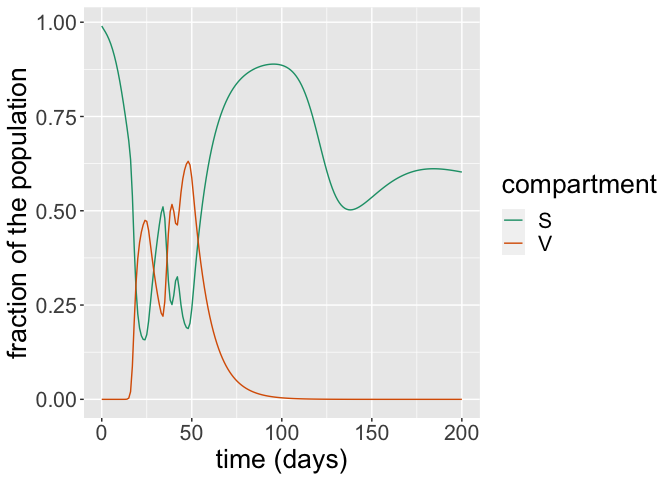
\includegraphics{SEIRD_contact_matrix_files/figure-latex/unnamed-chunk-8-1.pdf}

\begin{Shaded}
\begin{Highlighting}[]

\NormalTok{I\_data }\OtherTok{\textless{}{-}} \FunctionTok{filter}\NormalTok{(all\_results, age\_range}\SpecialCharTok{==}\StringTok{"75{-}80"}\NormalTok{, compartment}\SpecialCharTok{==}\StringTok{"I"}\NormalTok{)}
\NormalTok{data }\OtherTok{\textless{}{-}}\NormalTok{ I\_data}\SpecialCharTok{$}\NormalTok{value }\SpecialCharTok{*} \FunctionTok{sum}\NormalTok{(pops)}
\FunctionTok{dim}\NormalTok{(data) }\OtherTok{\textless{}{-}} \FunctionTok{c}\NormalTok{(}\FunctionTok{length}\NormalTok{(I\_data}\SpecialCharTok{$}\NormalTok{time)}\SpecialCharTok{/}\NormalTok{n\_bootstrap, n\_bootstrap)}
\NormalTok{quants }\OtherTok{\textless{}{-}} \FunctionTok{t}\NormalTok{(}\FunctionTok{apply}\NormalTok{(data, }\DecValTok{1}\NormalTok{, quantile, }\AttributeTok{probs=}\FunctionTok{c}\NormalTok{(}\FloatTok{0.05}\NormalTok{, }\FloatTok{0.5}\NormalTok{, }\FloatTok{0.95}\NormalTok{), }\AttributeTok{na.rm=}\ConstantTok{TRUE}\NormalTok{))}
\NormalTok{quants\_df }\OtherTok{\textless{}{-}} \FunctionTok{data.frame}\NormalTok{(quants)}
\NormalTok{quants\_df[}\StringTok{"time"}\NormalTok{] }\OtherTok{\textless{}{-}} \FunctionTok{seq}\NormalTok{(}\DecValTok{0}\NormalTok{, }\DecValTok{365}\NormalTok{, }\AttributeTok{by=}\DecValTok{1}\NormalTok{)}

\FunctionTok{ggplot}\NormalTok{(quants\_df, }\FunctionTok{aes}\NormalTok{(}\AttributeTok{x =}\NormalTok{ time)) }\SpecialCharTok{+}
  \FunctionTok{geom\_line}\NormalTok{(}\FunctionTok{aes}\NormalTok{(}\AttributeTok{y=}\NormalTok{X50.)) }\SpecialCharTok{+}
  \FunctionTok{geom\_ribbon}\NormalTok{(}\FunctionTok{aes}\NormalTok{(}\AttributeTok{ymin=}\NormalTok{X5., }\AttributeTok{ymax=}\NormalTok{X95.), }\AttributeTok{fill=}\StringTok{"blue"}\NormalTok{, }\AttributeTok{alpha=}\FloatTok{0.5}\NormalTok{) }\SpecialCharTok{+}
  \FunctionTok{ylab}\NormalTok{(}\StringTok{"I compartment, age 75{-}80"}\NormalTok{)}
\end{Highlighting}
\end{Shaded}

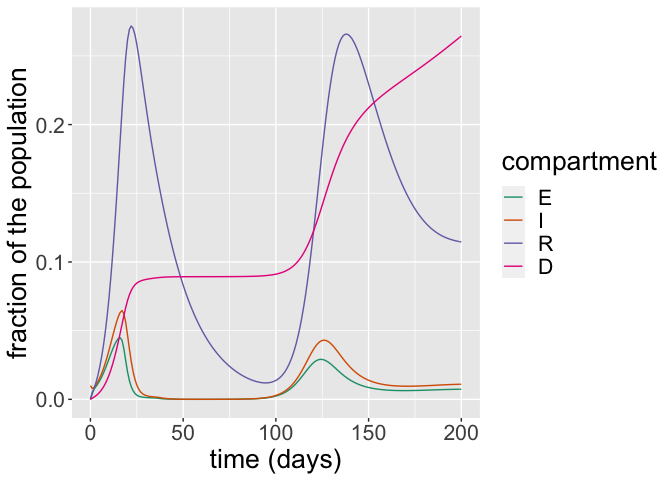
\includegraphics{SEIRD_contact_matrix_files/figure-latex/unnamed-chunk-8-2.pdf}

The results show that the while the shape of the epidemic trajectory
remains similar for all contact matrices in the bootstrap sample, the
number of people in the infected compartment exhibits significant
uncertainty, particularly near the peak of the epidemic.

Next, we perform the uncertainty analysis for the number in the
recovered compartment at the final time point, for all age groups.

\begin{Shaded}
\begin{Highlighting}[]

\NormalTok{data }\OtherTok{\textless{}{-}} \FunctionTok{filter}\NormalTok{(all\_results, compartment}\SpecialCharTok{==}\StringTok{"R"}\NormalTok{, time}\SpecialCharTok{==}\FloatTok{365.0}\NormalTok{)}

\FunctionTok{ggplot}\NormalTok{(data, }\FunctionTok{aes}\NormalTok{(}\AttributeTok{x=}\NormalTok{age\_range, }\AttributeTok{y=}\NormalTok{value}\SpecialCharTok{/}\NormalTok{pop\_fraction), l) }\SpecialCharTok{+}
  \FunctionTok{geom\_boxplot}\NormalTok{() }\SpecialCharTok{+}
  \FunctionTok{xlab}\NormalTok{(}\StringTok{"Age group"}\NormalTok{) }\SpecialCharTok{+}
  \FunctionTok{ylab}\NormalTok{(}\StringTok{"Proportion of age group ever infected"}\NormalTok{)}
\end{Highlighting}
\end{Shaded}

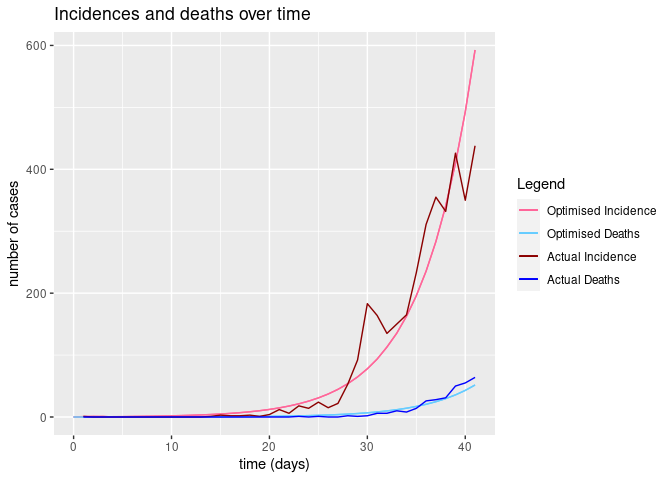
\includegraphics{SEIRD_contact_matrix_files/figure-latex/unnamed-chunk-9-1.pdf}
These results show that younger age groups suffer more infections. This
trend can be explained by the larger numbers of total contacts for
younger age groups, as observed in the contact matrices at the beginning
of this notebook.

Finally, we study the effects on death.

\begin{Shaded}
\begin{Highlighting}[]

\NormalTok{data }\OtherTok{\textless{}{-}} \FunctionTok{filter}\NormalTok{(all\_results, compartment}\SpecialCharTok{==}\StringTok{"D"}\NormalTok{, time}\SpecialCharTok{==}\FloatTok{365.0}\NormalTok{)}

\FunctionTok{ggplot}\NormalTok{(data, }\FunctionTok{aes}\NormalTok{(}\AttributeTok{x=}\NormalTok{age\_range, }\AttributeTok{y=}\NormalTok{value}\SpecialCharTok{/}\NormalTok{pop\_fraction), l) }\SpecialCharTok{+}
  \FunctionTok{geom\_boxplot}\NormalTok{() }\SpecialCharTok{+}
  \FunctionTok{xlab}\NormalTok{(}\StringTok{"Age group"}\NormalTok{) }\SpecialCharTok{+}
  \FunctionTok{ylab}\NormalTok{(}\StringTok{"Proportion of age group died"}\NormalTok{)}
\end{Highlighting}
\end{Shaded}

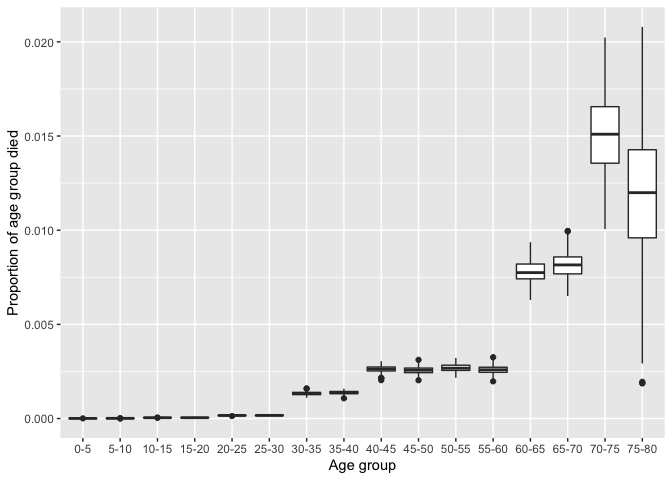
\includegraphics{SEIRD_contact_matrix_files/figure-latex/unnamed-chunk-10-1.pdf}
Although younger people are more likely to be infected in this
simulation, deaths occur mainly in the elderly, due to the
age-structured mortality parameter \(\mu\) described above. The
different bootstrap samples of the contact matrix result in a wide range
in the number of deaths, particularly in the 70--80 age groups.

\hypertarget{references}{%
\subsection*{References}\label{references}}
\addcontentsline{toc}{subsection}{References}

\hypertarget{refs}{}
\begin{CSLReferences}{1}{0}
\leavevmode\hypertarget{ref-ferguson2020report}{}%
Ferguson, Neil, Daniel Laydon, Gemma Nedjati Gilani, Natsuko Imai, Kylie
Ainslie, Marc Baguelin, Sangeeta Bhatia, et al. 2020. {``Report 9:
Impact of Non-Pharmaceutical Interventions (NPIs) to Reduce Covid19
Mortality and Healthcare Demand.''}

\leavevmode\hypertarget{ref-prem2021projecting}{}%
Prem, Kiesha, Kevin van Zandvoort, Petra Klepac, Rosalind M Eggo,
Nicholas G Davies, Centre for the Mathematical Modelling of Infectious
Diseases COVID-19 Working Group, Alex R Cook, and Mark Jit. 2021.
{``Projecting Contact Matrices in 177 Geographical Regions: An Update
and Comparison with Empirical Data for the COVID-19 Era.''} \emph{PLoS
Computational Biology} 17 (7): e1009098.

\leavevmode\hypertarget{ref-stayathome2021}{}%
UK government. 2021. {``{Stay at home: guidance for households with
possible or confirmed coronavirus (COVID-19) infection. Updated 2
December 2021.}''}
\url{https://www.gov.uk/government/publications/covid-19-stay-at-home-guidance/stay-at-home-guidance-for-households-with-possible-coronavirus-covid-19-infection}.

\leavevmode\hypertarget{ref-verity2020estimates}{}%
Verity, Robert, Lucy C Okell, Ilaria Dorigatti, Peter Winskill, Charles
Whittaker, Natsuko Imai, Gina Cuomo-Dannenburg, et al. 2020.
{``Estimates of the Severity of Coronavirus Disease 2019: A Model-Based
Analysis.''} \emph{The Lancet Infectious Diseases} 20 (6): 669--77.

\leavevmode\hypertarget{ref-xin2021estimating}{}%
Xin, Hualei, Yu Li, Peng Wu, Zhili Li, Eric HY Lau, Ying Qin, Liping
Wang, Benjamin J Cowling, Tim Tsang, and Zhongjie Li. 2021.
{``Estimating the Latent Period of Coronavirus Disease 2019
(COVID-19).''} \emph{Clinical Infectious Diseases: An Official
Publication of the Infectious Diseases Society of America}.

\end{CSLReferences}

\end{document}
